\section{Introduction}
%application use case
%company benefit
The profitability of a transport company, or any company for that matter, is closely linked to the efficiency with which it uses its resources.
% can command the scarce resources available to it.
In a transport company this roughly translates to
% usually takes the form of minimizing the costs made by
the use of its trucks and man hours, whilst fulfilling all service requirements.
%environment
A more efficient use of resources by transport companies will reduce the environmental impact of that industry, which for the U.S. has been estimated as 27\% of the total greenhouse gas emissions in 2013~\cite{inventory1990}.
%plug importance
The research that has been done on the vehicle routing problem (VRP) can help manage these challenges. \\

%research use case
Laporte defines the VRP concisely as `the problem of designing least-cost delivery routes from a depot to a set of geographically scattered customers, subject to side constraints'~\cite{laporte2009fifty}. It was first introduced by Dantzig and Ramser in 1959~\cite{dantzig1959truck} and has driven the development of exact algorithms and heuristics ever since. In practically no time after its introduction hundreds of models  and optimization methods were considered for various versions of the VRP. Today, many software packages exist on the market, all attempting to solve some of the real-world versions of the problem~\cite{toth2014vehicle}. \\

%points to make:
%1 There are many different types of problems
The economic incentives behind being able to solve real-world VRPs have produced many versions of the problem over the years, all catering to different operational realities. These  extensions of the VRP are often called rich vehicle routing problems (RVRPs).
%2 it is desirable to have a unifying framework for these problems
There is a need for a unifying solution framework for these RVRPs, since it will increase our understanding of the impact specific problem attributes have on our ability to find solutions. Furthermore, it will reduce the development time of solution methods for problems with new types problem attributes \cite{vidal2014unified}.\\

%3 Ropke has started in this direction
Progress has been made in creating heuristics that perform well on a broad class of problems \cite{vidal2014unified,pisinger2007general}.
%4 There is still a big class of problems that has been largely neglected namely vrpms
Still, in Drexl's comparison of commercial software and scientific research for modeling and solving VRPs he concludes: `models and algorithms for integrated and synchronized vehicle routing are still scarce: in almost all vehicle routing models and algorithms, the routes of the different vehicles are assumed to be independent of one another, so that modifying one route does not have any effects on other routes'. In \cite{drexl2012rich} the case is made that in a high number of cases this assumption does not hold. \\

%5 Vrptt are a usefull tool for modelling this class of problems
Problems with this interdependence attribute belong to the class of problems called vehicle routing problems with multiple synchronization constraints (VRPMS). These problems are of great practical relevance and quite hard to solve. In \cite{drexl2013applications} Drexl proposes and demonstrates the value of the vehicle routing problem with trailers and transshipment (VRPTT) as a general modeling tool for several classes of VRPMSs. Drexl solved small instances of the VRPTT using a branch-and-cut method \cite{drexl2014bandc}, but concludes that `a heuristic procedure for the VRPTT is needed, but still missing'.\\

%6 a heuristic is the way to go to solve this problem
VRP heuristics have gotten much attention. Exact algorithms have trouble solving even moderately sized VRPs and have a slow convergence rate \cite{cordeau2002guide}. Heuristics can be used to find high-quality solutions quickly for realistically-sized problems. They do not guarantee optimality though.
%7 A good attempt is to use ALNS since good result have been reached
The adaptive large neighborhood search (ALNS) heuristic is a promising optimization method \cite{pisinger2007general}. Good results have been achieved by applying it to a broad class of VRPs. Masson et al. have had good results applying it to the dial-a-ride problem with transfers in \cite{masson2014dial}, which is a problem that belongs to the class of VRPMSs . \\
 % They provided a sophisticated framework that speeds up feasibility checking.


%8 drexl's suggestion for heuristic approach to VRPTT
An outline of a heuristic approach to solving VRPMSs is given in \cite{drexl2014generic}. Drexl suggests a two-stage approach that is also used in \cite{drexl2013simultaneous} for simultaneous vehicle and crew routing and scheduling.

% The optimization method developed in this thesis uses a simplified version of the ALNS, namely a variable neighborhood search (VNS).
% .. VRPTTMu


\subsection{About TransMission}
The inducement to start working on the VRPTT has been provided by a company called TransMission.
TransMission is the largest cooperation of independent transport and distribution companies in the Benelux. The transport and distribution companies within the TransMission group work under one name. These organizations are also independent operations, and many of them are family companies. TransMission has 18 depots whereof thirteen are located in The Netherlands, four in Belgium and one in Luxembourg. Each depot services a region, such that  they cover the Benelux together. In Figure~\ref{fig:regions} the separate regions can be seen on the map. \\

\begin{figure}[!ht]
  \centering
    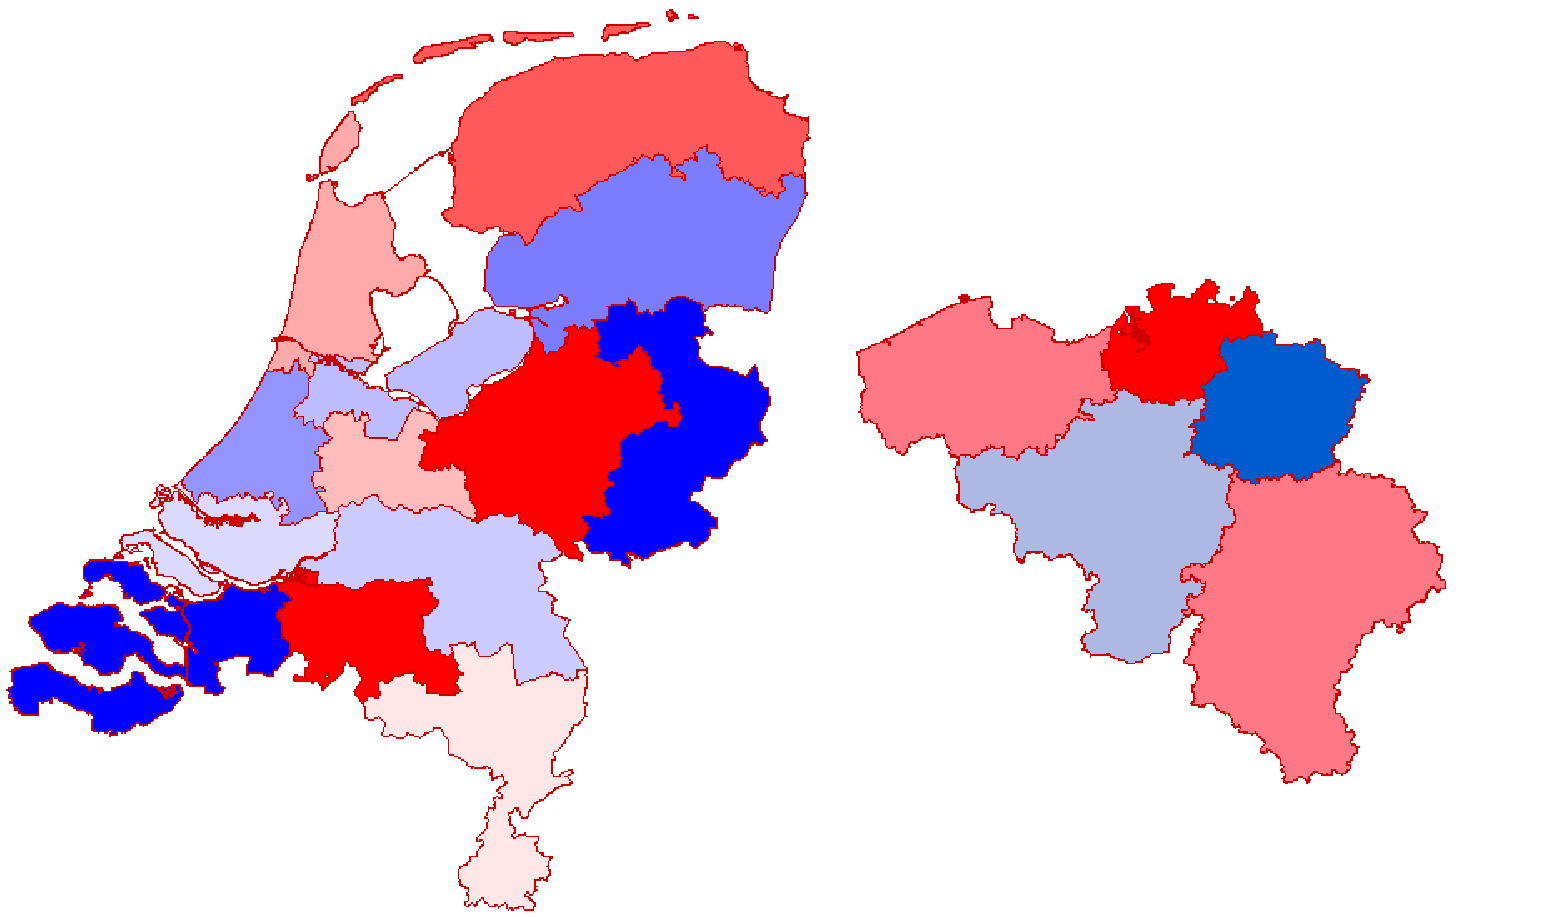
\includegraphics[width=0.8\textwidth]{img/transmission_regions.pdf}
  \caption{The regions serviced by the transport and distribution companies within the TransMission group . The depot located in Luxembourg services the South-East of Belgium and the whole of Luxembourg.}
  \label{fig:regions}
\end{figure}

TransMission uses different types of trucks and trailers and many of their depots can be used as cross-docks.
Line hauls are used to move cargo between depots during nights. Depots pick up and deliver the cargo in their service regions during days. There is a long-term centrally planned set of line hauls. There is also a set of line hauls that is planned daily  by the depots themselves.
TransMission would like to to produce its transport plans every day using all information available to the depots.
 % optimize its planning centrally on per day basis.
To achieve this, producing the transport plan needs to become automated.



\subsection{Scope}

TransMission's problem is an extremely rich one.
The first step to solve a problem is to model it properly.
% The first step to solving a problem is properly modeling it.
It is a pick up and delivery problem without fixed assignments of trailers to lorries where goods can be transfered between vehicles before they reach their destination.
% Furthermore, goods can be transfered from one vehicle to another before it reaches its destination.
\\


In \cite{masson2013adaptive} results are reported on the pickup and delivery problem with transshipments.
In this paper the available fleet is homogeneous and does not contain trailers.
The VRPTT considered in \cite{drexl2007some} only deals with collecting one homogeneous good, instead of picking up and delivering various goods to various locations.
Both works do not cover all features of TransMission's problem.
Of these two models, the VRPTT has been estimated to be the best basis for a model for TransMission's problem.
Its potential to model a wide class of problems has already been demonstrated in \cite{drexl2013applications}.\\

% The main reason TransMissions problem is hardThe loose coupling of trailers and lorries combined with load transfers and a heterogeneous fleet make TransMissions problem difficult to model.

% The VRPTT proposed by Drexl in \cite{drexl2007some} as the best candidate to serve as a basis for the solution to TransMission's problem. Its potential to model a wide class of problems has already been demonstrated in \cite{drexl2013applications}.

Powerful algorithms for solving the VRPTT do not exist yet \cite{drexl2014bandc}.
Stochastic optimization methods and/or heuristics may offer solutions in cases where solving problems exactly is too slow.
Developing such an algorithm is therefore the most logical first step towards solving TransMission's problem. This task is the scope of this thesis. The optimization method will be a simplified version of the ALNS, namely a variable neighborhood search (VNS). The ALNS  has shown promising results on large instances in \cite{masson2013adaptive}.\\

 How the results of this thesis will be used to automate the production of transport plans for TransMission is outside the scope of this thesis.




\subsection{Methodology}
%work transmission
A week was spent within TransMission to work in different departments in order to gain  domain knowledge.
The problem was defined and the scope was determined in collaboration with TransMission.\\

%programming
The python programming language \cite{vanpython} was used to make the algorithm since it allows for rapid prototyping and easy visualizations.
The Numpy package \cite{numpy} was used for fast array computations.
 The  Numba library \cite{analytics2014numba} was used to speed up performance-critical parts of the algorithm.
 Instances provided in \cite{drexl2007some,drexl2011branch} were used to analyze the performance of the algorithm.

\subsection{Outline}
This section provides the problem under consideration with context.
Section \ref{chap:The Problem} explains the problem and formulates the model.
 % the problem and describe its complexities.
%We look at the theory on which our optimization method is based in chapter \ref{chap:Theory}.
In Section \ref{chap:Optimization} all parts of the optimization method are explained.
 % that was used to generate results.
The test methods and the results that were produced by the optimization method are described and interpreted in Section \ref{chap:Tests and Results}.
In Section \ref{chap:Discussion and Future Work} conclusions are drawn and  Section \ref{chap:future-work} outlines promising  directions of this area of research.
 % about future directions and/or opport of this line of research.
% \todo{update this subsection in the end}
